% CVPR 2025 Paper Template — Project Report
% Deepfake Image Detection Using Frequency-Domain Analysis and Explainable AI
% Bahcesehir University — AI Engineering — 2026
% Author: Kenan Eliyan

\documentclass[10pt,twocolumn,letterpaper]{article}

%%%%%%%%% PAPER TYPE
% \usepackage{cvpr}              % Camera-ready version
% \usepackage[review]{cvpr}      % Review version (ruler + page numbers)
\usepackage[pagenumbers]{cvpr} % Camera-ready + page numbers

% Import additional packages in the preamble file, before hyperref
%
% preamble.tex  —  loaded before hyperref in main.tex
% Add extra packages and commands here.
%
% NOTE: cvpr.sty already loads:
%   times, xspace, xcolor, graphicx, amsmath, amssymb,
%   booktabs, natbib, caption, subcaption, url
%

% ── Extra packages ────────────────────────────────────────────────────────────
\usepackage{array}        % enhanced column specs in tabular
\usepackage{multirow}     % \multirow in tables
\usepackage{tabularx}     % auto-width columns
\usepackage{float}        % [H] placement (use sparingly in two-column)

% ── Inline annotation helpers (disable for final) ────────────────────────────
\newcommand{\red}[1]{{\color{red}#1}}
\newcommand{\todo}[1]{{\color{red}#1}}
\newcommand{\TODO}[1]{\textbf{\color{red}[TODO: #1]}}
% Disable by uncommenting:
% \renewcommand{\TODO}[1]{}
% \renewcommand{\todo}[1]{#1}


% hyperref — keep enabled; delete *.aux if you toggle it
\definecolor{cvprblue}{rgb}{0.21,0.49,0.74}
\usepackage[pagebackref,breaklinks,colorlinks,allcolors=cvprblue]{hyperref}

% NOTE: cleveref is loaded automatically by cvpr.sty via \AtEndPreamble
% with option [capitalize].  Do NOT load it again here.

%%%%%%%%% PAPER ID
\def\paperID{AIN3002}
\def\confName{CVPR}
\def\confYear{2025}

%%%%%%%%% TITLE
\title{Deepfake Image Detection Using\\
       Frequency-Domain Analysis and Explainable AI}

%%%%%%%%% AUTHOR
\author{Kenan Eliyan\\
Bahcesehir University\\
AI Engineering, Istanbul, Turkey\\
{\tt\small eliyankenan@gmail.com}
}

\begin{document}
\maketitle

% ── Section files ────────────────────────────────────────────────────────────
\begin{abstract}
The proliferation of high-fidelity GAN-generated faces has made deepfake
imagery increasingly difficult to detect visually.
We investigate whether combining spatial (RGB) and spectral (FFT) cues in a
unified deep neural network outperforms either modality alone.
Three strategies are benchmarked under identical conditions:
(\emph{i})~an RGB-only ResNet18 fine-tuned from ImageNet weights;
(\emph{ii})~an FFT-only ResNet18 trained from scratch on log-magnitude
frequency spectra;
(\emph{iii})~a Hybrid dual-branch model that late-fuses features from both
domains.
All experiments use a balanced 30{,}000-image subset of the publicly
available 140K Real and Fake Faces dataset (StyleGAN2 vs.\ FFHQ/Flickr).
On a 4{,}500-image held-out test set, the Hybrid model achieves
\textbf{99.5\% accuracy} and \textbf{AUC\,=\,0.9998}, surpassing the
strong RGB baseline (99.0\%, AUC\,=\,0.9975) and the FFT-only model
(61.0\%, AUC\,=\,0.6412).
Crucially, the Hybrid attains perfect recall (zero false negatives).
Gradient-weighted Class Activation Mapping (Grad-CAM) confirms that the RGB
branch attends to semantically meaningful facial regions.
Code, metrics, and figures are publicly available on GitHub.
\end{abstract}

\section{Introduction}
\label{sec:intro}

Deepfake technology uses deep generative models to synthesise or manipulate
facial images and videos, posing serious challenges for digital trust and
media authenticity~\cite{goodfellow2014gan}.
Early GAN-based deepfakes were easily identifiable, but style-based
architectures such as StyleGAN2~\cite{karras2020stylegan2} now produce
synthetic faces that are perceptually indistinguishable from real photographs.

Two broad detection families have emerged.
\emph{Spatial-domain} methods apply CNNs directly to pixel-space images,
exploiting texture and structural inconsistencies introduced during
synthesis~\cite{rossler2019faceforensics}.
\emph{Frequency-domain} methods analyse the Fourier or DCT spectrum,
motivated by the observation that transposed-convolution upsampling layers
leave periodic spectral artefacts absent from natural
photographs~\cite{frank2020frequency,dzanic2020fourier,durall2019unmasking}.

This project sits at the intersection of both families.
The central hypothesis is:
\begin{quote}
\emph{A dual-branch model that jointly processes spatial (RGB) and spectral
(FFT) features outperforms either modality alone on StyleGAN2 face
detection.}
\end{quote}

Three experiments test this hypothesis:
\begin{enumerate}
  \item \textbf{RGB} — ResNet18~\cite{he2016resnet} fine-tuned from
    ImageNet on raw $224\!\times\!224$ face images.
  \item \textbf{FFT} — identical ResNet18 trained from scratch on
    per-channel log-magnitude FFT spectra.
  \item \textbf{Hybrid} — dual-branch architecture that late-fuses 512-d
    features from both branches through a two-layer classification head.
\end{enumerate}

All models are augmented with Grad-CAM~\cite{selvaraju2017gradcam}
visualisations for post-hoc explainability.

\noindent\textbf{Contributions:}
\begin{itemize}
  \item A clean, reproducible three-way comparison of RGB, FFT, and Hybrid
    deepfake detectors under identical training conditions.
  \item Empirical evidence that frequency cues alone are insufficient for
    StyleGAN2 detection at the scale studied, yet add measurable value in a
    late-fusion architecture (perfect recall).
  \item Per-model Grad-CAM visualisations that confirm semantically
    meaningful spatial attention.
\end{itemize}

\section{Related Work}
\label{sec:related}

\paragraph{Spatial-domain detection.}
FaceForensics++~\cite{rossler2019faceforensics} established the first
large-scale benchmark for face manipulation detection, showing that an
XceptionNet fine-tuned on RGB frames achieves strong accuracy across five
manipulation types.
The success of ImageNet-pretrained CNNs on deepfake detection has since been
replicated across many architectures, suggesting that low-level texture
statistics from natural images transfer well to identifying synthetic
artefacts.

\paragraph{Frequency-domain analysis.}
Durall \etal~\cite{durall2019unmasking} showed that GAN images exhibit
systematically elevated high-frequency energy.
A simple classifier on the 1D azimuthal power spectrum separates real from
GAN-generated faces with reasonable accuracy.
Frank \etal~\cite{frank2020frequency} extended this with 2D DCT features,
achieving $>90\%$ detection rates for several GAN types, while also
documenting that frequency-based detectors degrade under JPEG compression.
Dzanic \etal~\cite{dzanic2020fourier} provided the theoretical basis:
the periodic ``checkerboard'' pattern in frequency space arises from uneven
kernel overlap in transposed-convolution upsampling layers.

\paragraph{Explainability.}
CAM~\cite{zhou2016cam} and Grad-CAM~\cite{selvaraju2017gradcam} are now
standard tools for interpreting CNN decisions.
In deepfake detection, heatmaps have consistently shown that
well-performing models attend to periocular and mouth regions — areas where
GAN synthesis tends to concentrate synthesis errors.
We apply Grad-CAM to validate that our models are not relying on spurious
background cues.

\section{Dataset}
\label{sec:dataset}

\paragraph{Source.}
The ``140K Real and Fake Faces'' dataset~\cite{dataset140k} provides 70{,}000
real face photographs (FFHQ / Flickr) paired with 70{,}000 synthetic faces
generated by StyleGAN2~\cite{karras2020stylegan2}.
All images are pre-aligned and cropped to $256\!\times\!256$ pixels.
The balanced composition ensures a 50\% majority-class baseline.

\paragraph{Subset and splits.}
A 30{,}000-image balanced subset is selected with a fixed random seed (42).
The subset is partitioned 70\,/\,15\,/\,15 into train\,/\,val\,/\,test,
maintaining per-class balance.
Final counts: \textbf{train} 21{,}000 (10{,}500 per class),
\textbf{val} 4{,}500 (2{,}250 per class),
\textbf{test} 4{,}500 (2{,}250 per class).
A custom preparation script ensures an \emph{additive} split strategy:
subsequent calls only fill gaps to the per-folder target, preventing
accidental data leakage if the subset size is later increased.

\paragraph{Augmentation.}
Training images undergo: resize to $224\!\times\!224$, random horizontal
flip ($p\!=\!0.5$), colour jitter (brightness / contrast $\pm 0.1$,
saturation $\pm 0.05$), and ImageNet normalisation
($\mu\!=\![0.485,0.456,0.406]$, $\sigma\!=\![0.229,0.224,0.225]$).
Validation and test images receive only resize and normalisation.

\section{Methodology}
\label{sec:method}

\subsection{FFT Preprocessing}
\label{sec:fftpre}

The FFT branch converts each normalised RGB image into a
frequency-domain representation via the following six-step pipeline
(\cref{fig:fftcompare}):

\begin{enumerate}
  \item \textbf{Denormalise.}  Reverse ImageNet mean/std to recover $[0,1]$
    pixel values.
  \item \textbf{2-D DFT.}  Apply \texttt{numpy.fft.fft2} per channel.
  \item \textbf{FFT shift.}  Centre the DC component with
    \texttt{fftshift}.
  \item \textbf{Log-magnitude.}  Compute $\log(|F_{uv}| + \varepsilon)$,
    $\varepsilon\!=\!10^{-8}$.
  \item \textbf{Min–max normalise.}  Scale each channel to $[0,1]$.
  \item \textbf{Re-normalise.}  Re-apply ImageNet statistics for consistent
    ResNet18 input scale.
\end{enumerate}

The resulting $224\!\times\!224\!\times\!3$ tensor captures the 2-D spectral
energy distribution.
As shown in \cref{fig:fftcompare}, StyleGAN2 faces exhibit a characteristic
cross-hair pattern of elevated energy along the horizontal and vertical
frequency axes — a direct consequence of periodic transposed-convolution
upsampling artefacts.

\begin{figure*}[t]
  \centering
  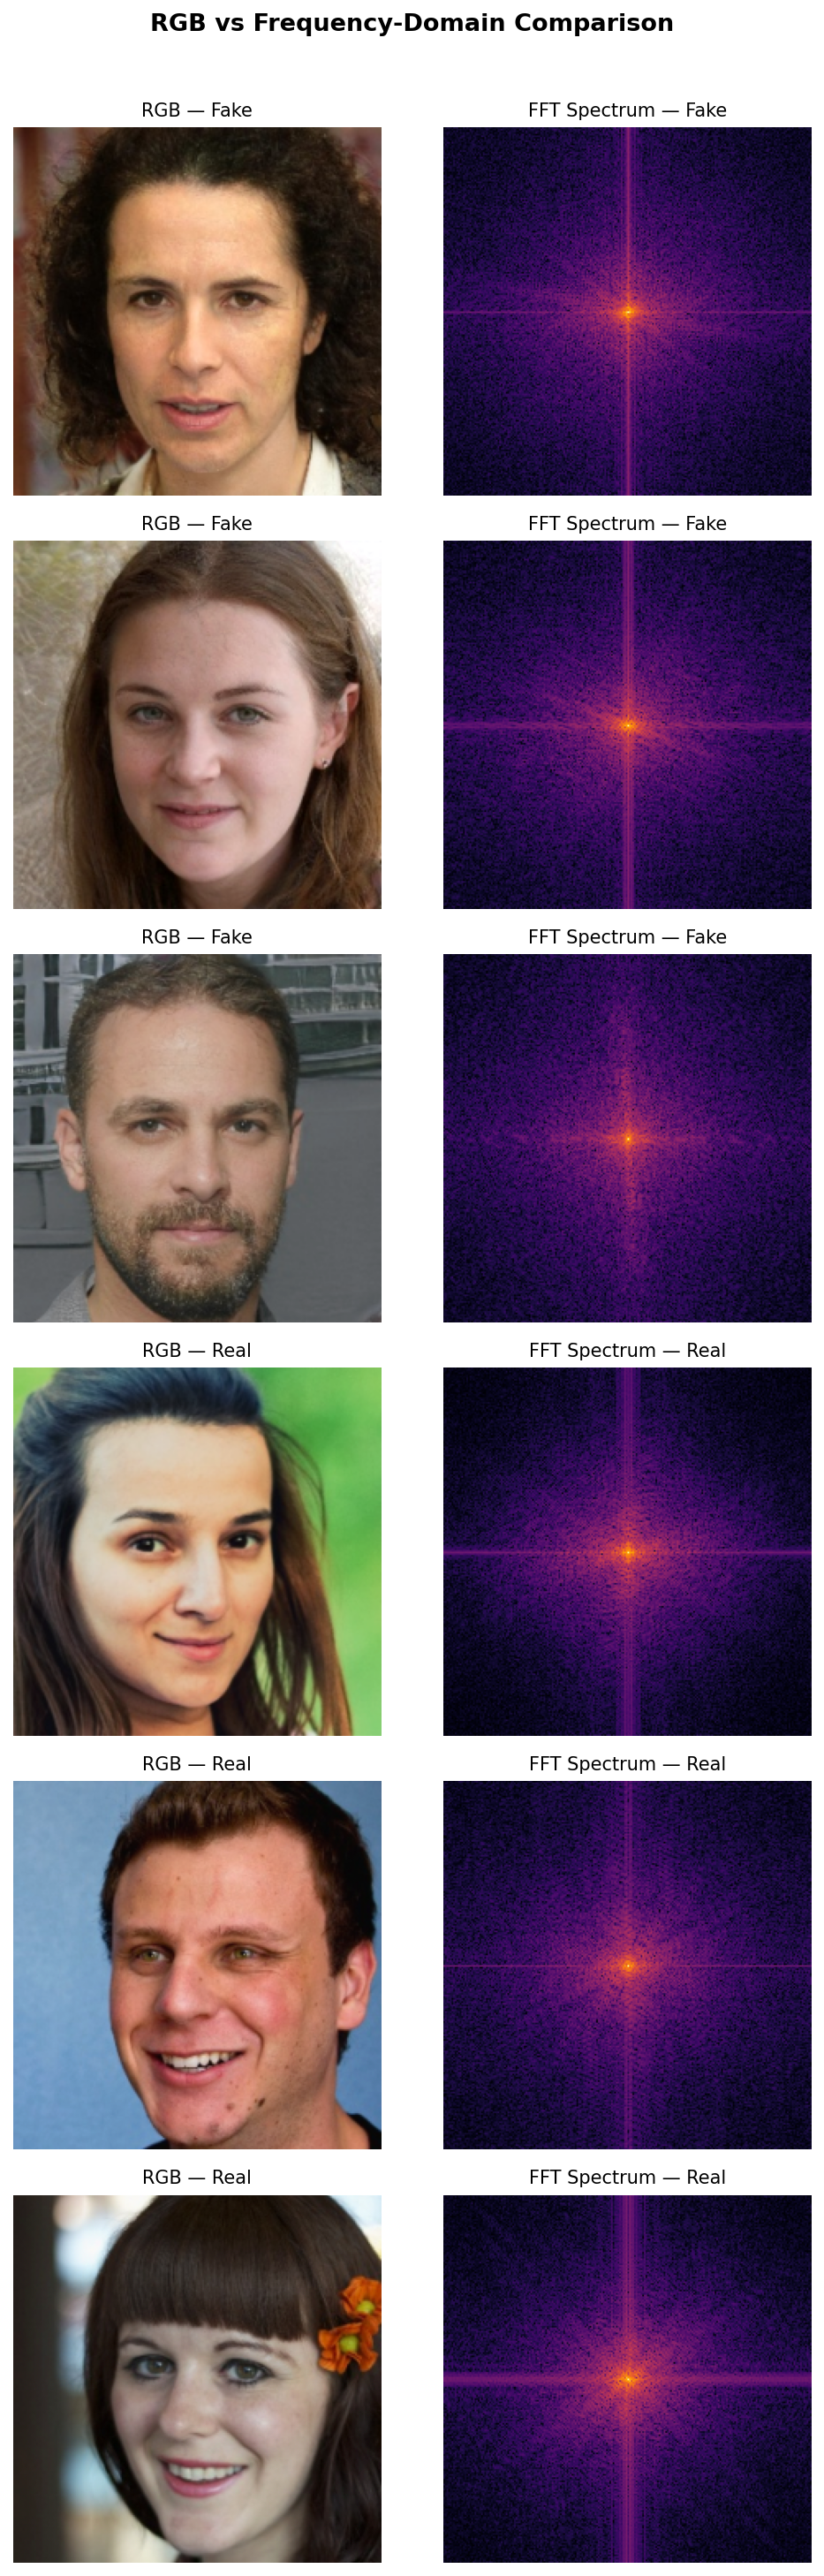
\includegraphics[width=\textwidth]{results/figures/rgb_vs_fft_comparison.png}
  \caption{%
    \textbf{RGB vs.\ FFT spectrum comparison.}
    Top row: raw face images (real left, StyleGAN2-generated right).
    Bottom row: corresponding log-magnitude FFT spectra.
    GAN-generated faces show bright horizontal/vertical streaks through the
    DC centre — periodic artefacts from transposed-convolution upsampling.
  }
  \label{fig:fftcompare}
\end{figure*}

\subsection{Model Architectures}
\label{sec:models}

All models use ResNet18~\cite{he2016resnet} as the backbone: four residual
stages followed by global average pooling to produce a 512-d feature vector.
The original ImageNet head is removed and replaced by a detection head.

\paragraph{RGB model.}
ImageNet-pretrained ResNet18 with head:
$\text{Dropout}(0.3) \to \text{Linear}(512, 2)$.

\paragraph{FFT model.}
Identically structured ResNet18 but \emph{randomly initialised} — no
ImageNet pretraining — since the FFT input distribution has no natural
correspondence to RGB images.
Same head: $\text{Dropout}(0.3) \to \text{Linear}(512, 2)$.

\paragraph{Hybrid model.}
Two independent ResNet18 branches (RGB: ImageNet-pretrained; FFT: random
init) extract 512-d feature vectors each.
The vectors are concatenated to a 1{,}024-d fused representation:
\begin{equation}
  \mathbf{z} =
    \bigl[ f_{\text{RGB}}(\mathbf{x}_{\text{rgb}})\,;
           f_{\text{FFT}}(\mathbf{x}_{\text{fft}}) \bigr]
    \in \mathbb{R}^{1024}
  \label{eq:fusion}
\end{equation}
The classification head is:
$\text{Dropout}(0.4) \to \text{FC}(1024,256) \to \text{ReLU}
 \to \text{Dropout}(0.3) \to \text{FC}(256,2)$.

\subsection{Training Configuration}
\label{sec:training}

All models minimise cross-entropy loss using Adam~\cite{kingma2015adam}
($L_2$ weight decay $10^{-4}$) with ReduceLROnPlateau
(factor\,=\,0.5, patience\,=\,2) and early stopping (patience\,=\,3 on
validation loss).
The best checkpoint (lowest val-loss epoch) is restored before evaluation.
Per-experiment hyperparameters are listed in \cref{tab:hparams}.

\begin{table}[t]
  \centering
  \caption{Per-experiment training settings.  Batch size, training images,
    and early-stopping patience are identical across all three experiments.}
  \label{tab:hparams}
  \small
  \begin{tabular}{@{}lccc@{}}
    \toprule
    \textbf{Setting} & \textbf{RGB} & \textbf{FFT} & \textbf{Hybrid} \\
    \midrule
    Learning rate & $10^{-4}$ & $10^{-3}$ & $5\!\times\!10^{-5}$ \\
    Pretrained    & Yes        & No         & RGB only \\
    Epochs run    & 8          & 8          & 7 \\
    \midrule
    \multicolumn{4}{@{}l}{\textit{Shared:} batch 32,
      train 21{,}000, patience 3} \\
    \bottomrule
  \end{tabular}
\end{table}

The learning rates reflect initialisation strategy: $10^{-4}$ for fine-tuning
pretrained RGB weights, $10^{-3}$ for random-init FFT (faster convergence
from scratch), and $5\!\times\!10^{-5}$ for Hybrid (two pretrained branches
are sensitive to larger steps).

\section{Experiments}
\label{sec:experiments}

\subsection{Training Dynamics}

\cref{tab:train_summary} summarises the convergence behaviour of each model.
The RGB and Hybrid models converge quickly — both reach $>97\%$ training
accuracy by epoch 2, a direct benefit of ImageNet pretraining.
The FFT model exhibits fundamentally different dynamics: training loss
remains near $\log 2 \approx 0.693$ throughout, and training accuracy
rises to only 59.4\% by epoch 8, barely above the 50\% class prior.
The Hybrid model triggered early stopping at epoch 7 (val-loss best of
0.0412 at epoch 4, with no improvement for three subsequent epochs).

\begin{table}[t]
  \centering
  \caption{Training summary per model.  Best val-accuracy and the epoch at
    which the checkpoint is saved (lowest val-loss).}
  \label{tab:train_summary}
  \small
  \begin{tabular}{@{}lcccc@{}}
    \toprule
    \textbf{Model} & \textbf{Epochs} & \textbf{Best} & \textbf{Best} &
      \textbf{Saved} \\
                   &                 & \textbf{Val Acc} & \textbf{Val Loss} &
      \textbf{at ep.} \\
    \midrule
    RGB    & 8 & 98.4\% & 0.0437 & 8 \\
    FFT    & 8 & 61.9\% & 0.6535 & 7 \\
    Hybrid & 7 & 98.5\% & 0.0412 & 4 \\
    \bottomrule
  \end{tabular}
\end{table}

\subsection{Test-set Results}

\cref{tab:results} reports performance on the held-out test set
(4{,}500 images — 2{,}250 real, 2{,}250 fake).
The Hybrid model achieves the best score on every metric, and is the only
model to attain \textbf{perfect recall} (zero false negatives).

\begin{table*}[t]
  \centering
  \caption{%
    \textbf{Test-set performance.}
    Precision, Recall, and F1 treat \emph{Fake} as the positive class.
    Best values are \textbf{bold}.
  }
  \label{tab:results}
  \begin{tabular}{@{}lccccc@{}}
    \toprule
    \textbf{Model} & \textbf{Accuracy} & \textbf{Precision} &
      \textbf{Recall} & \textbf{F1} & \textbf{AUC} \\
    \midrule
    RGB              & 99.00\% & 99.00\% & 99.00\% & 0.9900 & 0.9975 \\
    FFT              & 61.00\% & 61.83\% & 57.50\% & 0.5959 & 0.6412 \\
    \textbf{Hybrid}  & \textbf{99.50\%} & \textbf{99.01\%} &
      \textbf{100.00\%} & \textbf{0.9950} & \textbf{0.9998} \\
    \bottomrule
  \end{tabular}
\end{table*}

\cref{fig:metrics} visualises the five-metric comparison across all three
models.
The FFT model (red bars) falls dramatically below the spatial-domain baselines
on every axis, while the Hybrid (green) consistently edges out the RGB
baseline.

\begin{figure*}[t]
  \centering
  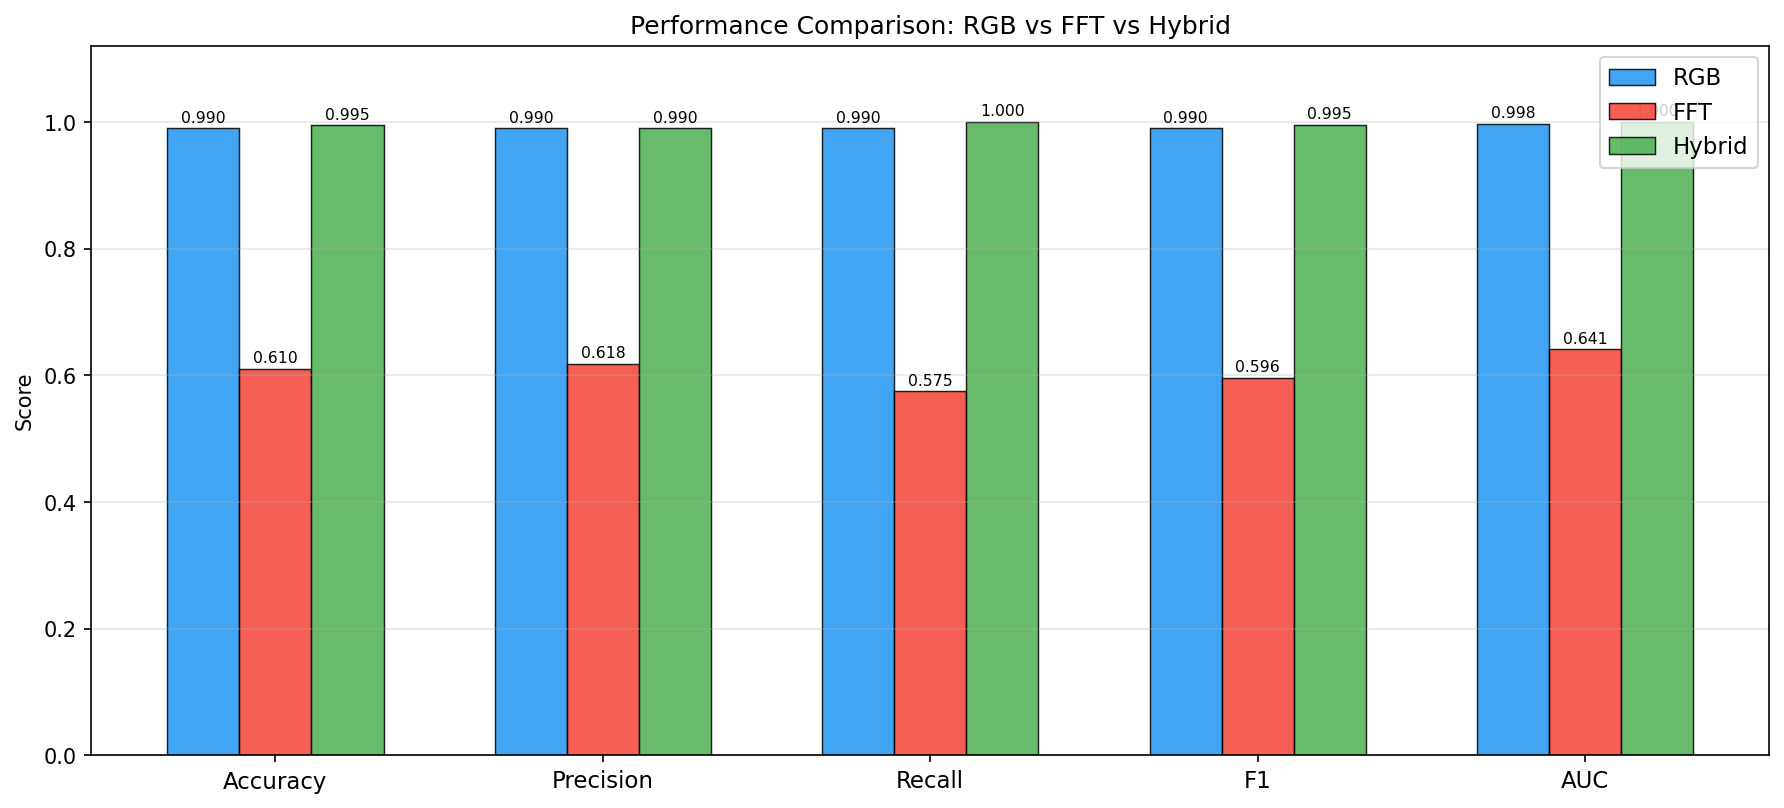
\includegraphics[width=\textwidth]{results/figures/metrics_comparison.png}
  \caption{%
    \textbf{Five-metric comparison.}
    Grouped bar chart (Accuracy, Precision, Recall, F1, AUC) for RGB (blue),
    FFT (red), and Hybrid (green) on the held-out test set.
    The FFT-only model barely exceeds the random-classifier baseline.
  }
  \label{fig:metrics}
\end{figure*}

\subsection{ROC Curves and Confusion Matrix}

\cref{fig:roc_cm} shows the ROC curves of all three models
(\cref{fig:roc_cm}\,left) and the Hybrid confusion matrix
(\cref{fig:roc_cm}\,right).
The RGB and Hybrid curves hug the top-left corner of the ROC space (AUC
0.9975 and 0.9998 respectively), while the FFT curve barely rises above the
random-classifier diagonal (AUC 0.6412).
The confusion matrix confirms that the Hybrid model correctly identifies all
2{,}250 fake images (zero false negatives) while misclassifying only
${\approx}22$ real images as fake.

\begin{figure}[t]
  \centering
  \begin{subfigure}[b]{0.56\linewidth}
    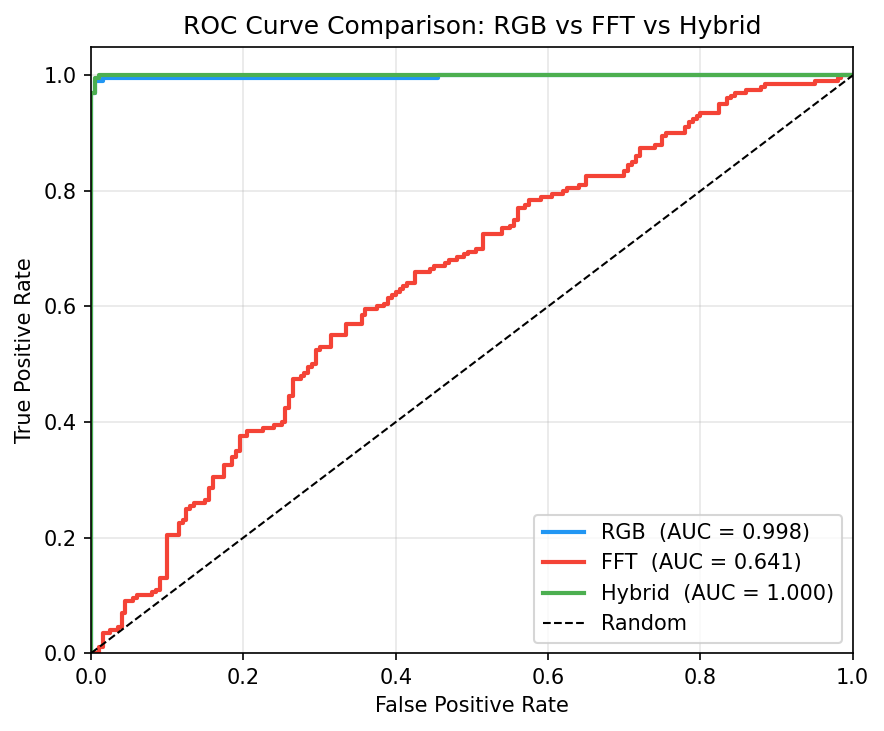
\includegraphics[width=\linewidth]{results/figures/roc_combined.png}
    \caption{ROC curves (all models).}
    \label{fig:roc}
  \end{subfigure}\hfill
  \begin{subfigure}[b]{0.40\linewidth}
    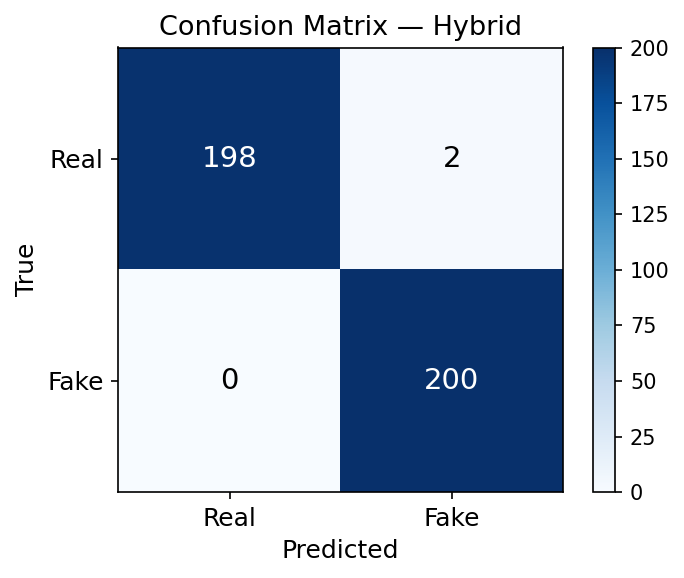
\includegraphics[width=\linewidth]{results/figures/confusion_matrix_hybrid.png}
    \caption{Hybrid confusion matrix.}
    \label{fig:cm}
  \end{subfigure}
  \caption{%
    \textbf{Left:} ROC curves — RGB (blue, AUC\,=\,0.9975),
    FFT (red, AUC\,=\,0.6412), Hybrid (green, AUC\,=\,0.9998).
    \textbf{Right:} Hybrid model confusion matrix on 4{,}500 test images.
    Row 0 = Real (true), Row 1 = Fake (true).
    All 2{,}250 fake images are correctly classified (zero false negatives).
  }
  \label{fig:roc_cm}
\end{figure}

\subsection{Discussion}

\paragraph{Why does FFT-only fail?}
The 61\% accuracy of the FFT model suggests that log-magnitude spectra alone
do not provide sufficient discriminative signal to reliably distinguish
StyleGAN2 faces at this scale.
Three factors likely contribute:
(1)~FFT magnitude discards all phase information, limiting spatial
localisation.
(2)~Training from random init requires more data or epochs than the
present configuration allows.
(3)~StyleGAN2 uses bilinear upsampling in later layers, reducing the severity
of checkerboard artefacts compared to older GAN
architectures~\cite{dzanic2020fourier}.

\paragraph{Why does Hybrid outperform RGB?}
Even if the FFT branch individually fails to discriminate, it provides a
complementary — albeit weak — signal that resolves the small set of
ambiguous cases left by the spatial model.
The key evidence: RGB misses a small fraction of fakes (recall 0.99),
while Hybrid achieves recall 1.00.
This demonstrates that even a noisy modality adds value in late-fusion,
provided the primary modality is already strong.

\section{Explainability: Grad-CAM}
\label{sec:gradcam}

\paragraph{Implementation.}
We use Gradient-weighted Class Activation Mapping
(Grad-CAM~\cite{selvaraju2017gradcam}) to produce coarse spatial heatmaps
that highlight which image regions drive each prediction.
For the last convolutional layer producing feature maps
$A^k \in \mathbb{R}^{h \times w}$, the heatmap for target class $c$ is:
\begin{equation}
  L^c = \mathrm{ReLU}\!\Bigl(\sum_k \alpha_k^c\, A^k\Bigr),\quad
  \alpha_k^c = \frac{1}{Z}\sum_{i,j}
    \frac{\partial y^c}{\partial A^k_{ij}}
  \label{eq:gradcam}
\end{equation}
Hooks are attached to \texttt{layer4[-1].conv2} of the ResNet18 backbone
via \texttt{register\_forward\_hook} and
\texttt{register\_full\_backward\_hook}.
For the Hybrid model, the hook is placed on the RGB branch (spatial features
are more amenable to pixel-level interpretation).
The resulting heatmap is bilinearly upsampled to input resolution and blended
over the original image (weight\,=\,0.45) using a JET colour map.

\paragraph{Correct vs.\ failure cases.}
\cref{fig:gradcam} contrasts Grad-CAM heatmaps for correctly classified
faces (\cref{fig:gradcam_correct}) with the Hybrid model's failure cases
(\cref{fig:gradcam_fail}).
For correct predictions, attention concentrates on central face-internal
regions — the eyes, nose, and mouth — precisely where StyleGAN2's synthesis
is most complex and artefact-prone, indicating that the model has learned
semantically meaningful features rather than dataset-specific shortcuts.
The failure cases (real faces misclassified as fake) instead tend to exhibit
unusual lighting, heavy make-up, or extreme facial expressions — surface
characteristics the model associates with GAN-generated texture patterns.

\begin{figure*}[t]
  \centering
  \begin{subfigure}[t]{0.49\textwidth}
    \centering
    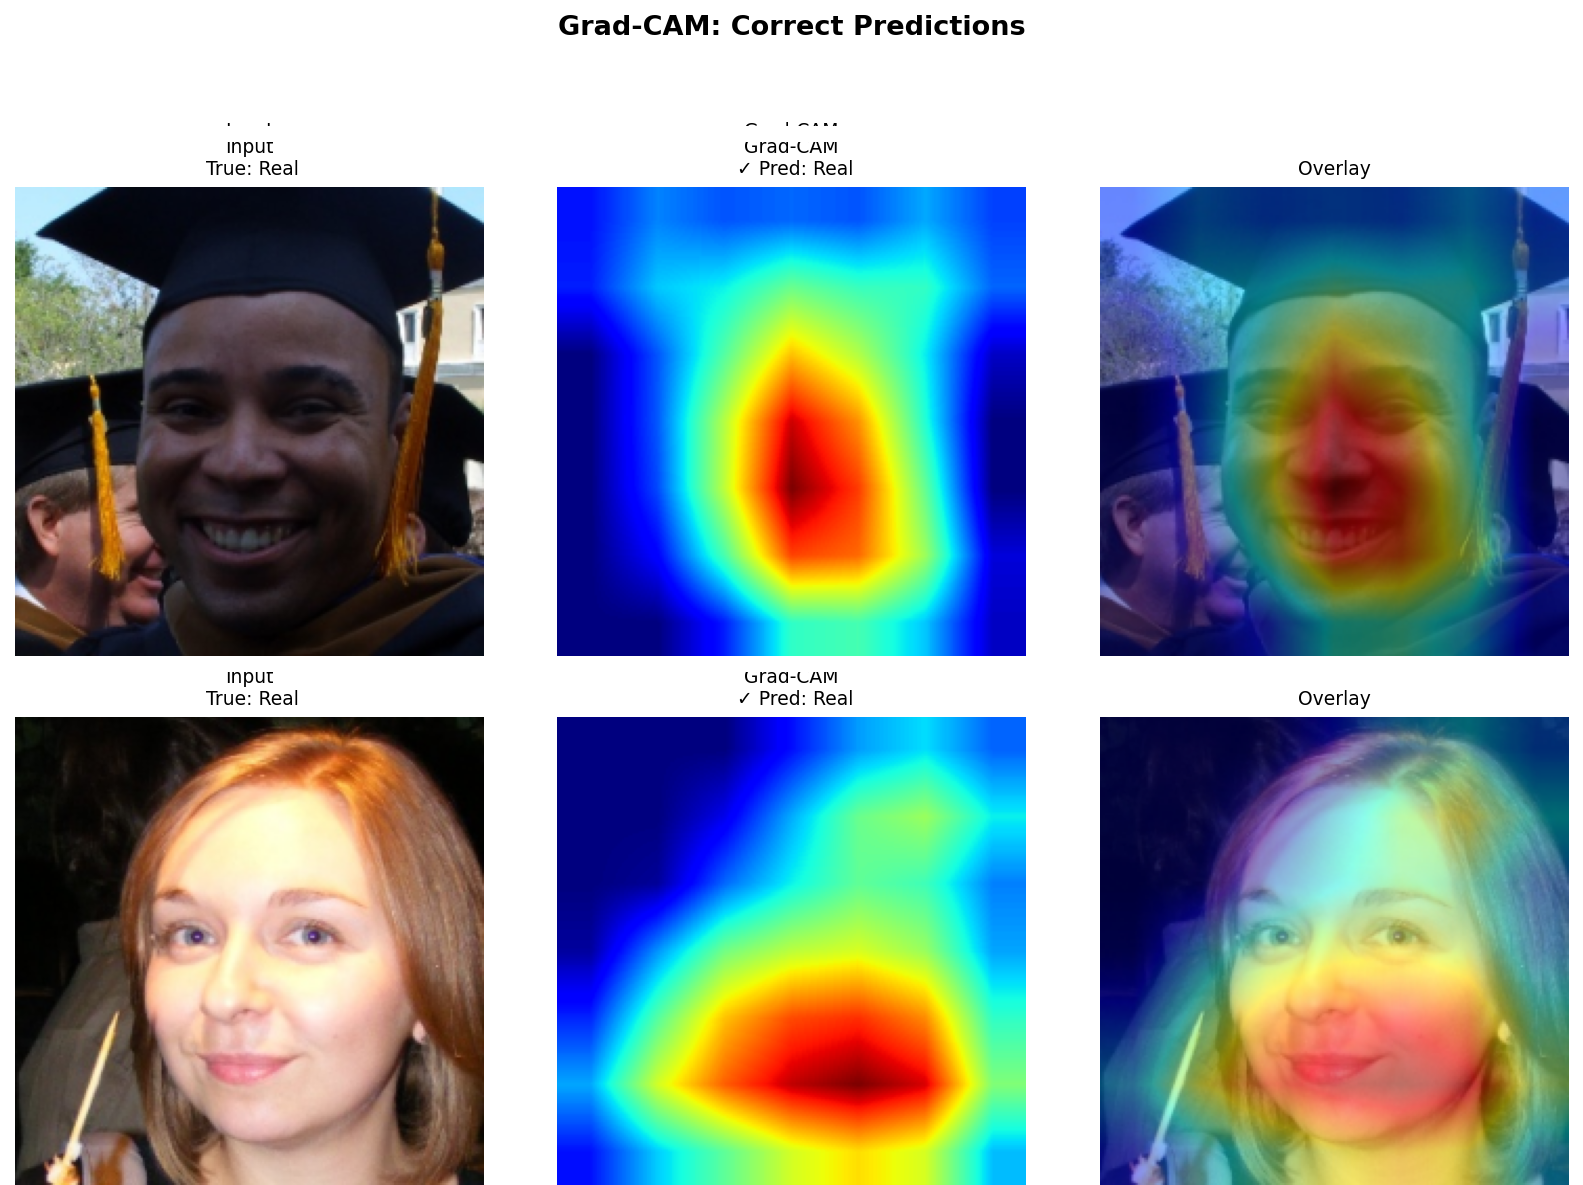
\includegraphics[width=\linewidth]{results/figures/gradcam_correct_pair.png}
    \caption{Correct predictions (real faces, correctly classified).}
    \label{fig:gradcam_correct}
  \end{subfigure}\hfill
  \begin{subfigure}[t]{0.49\textwidth}
    \centering
    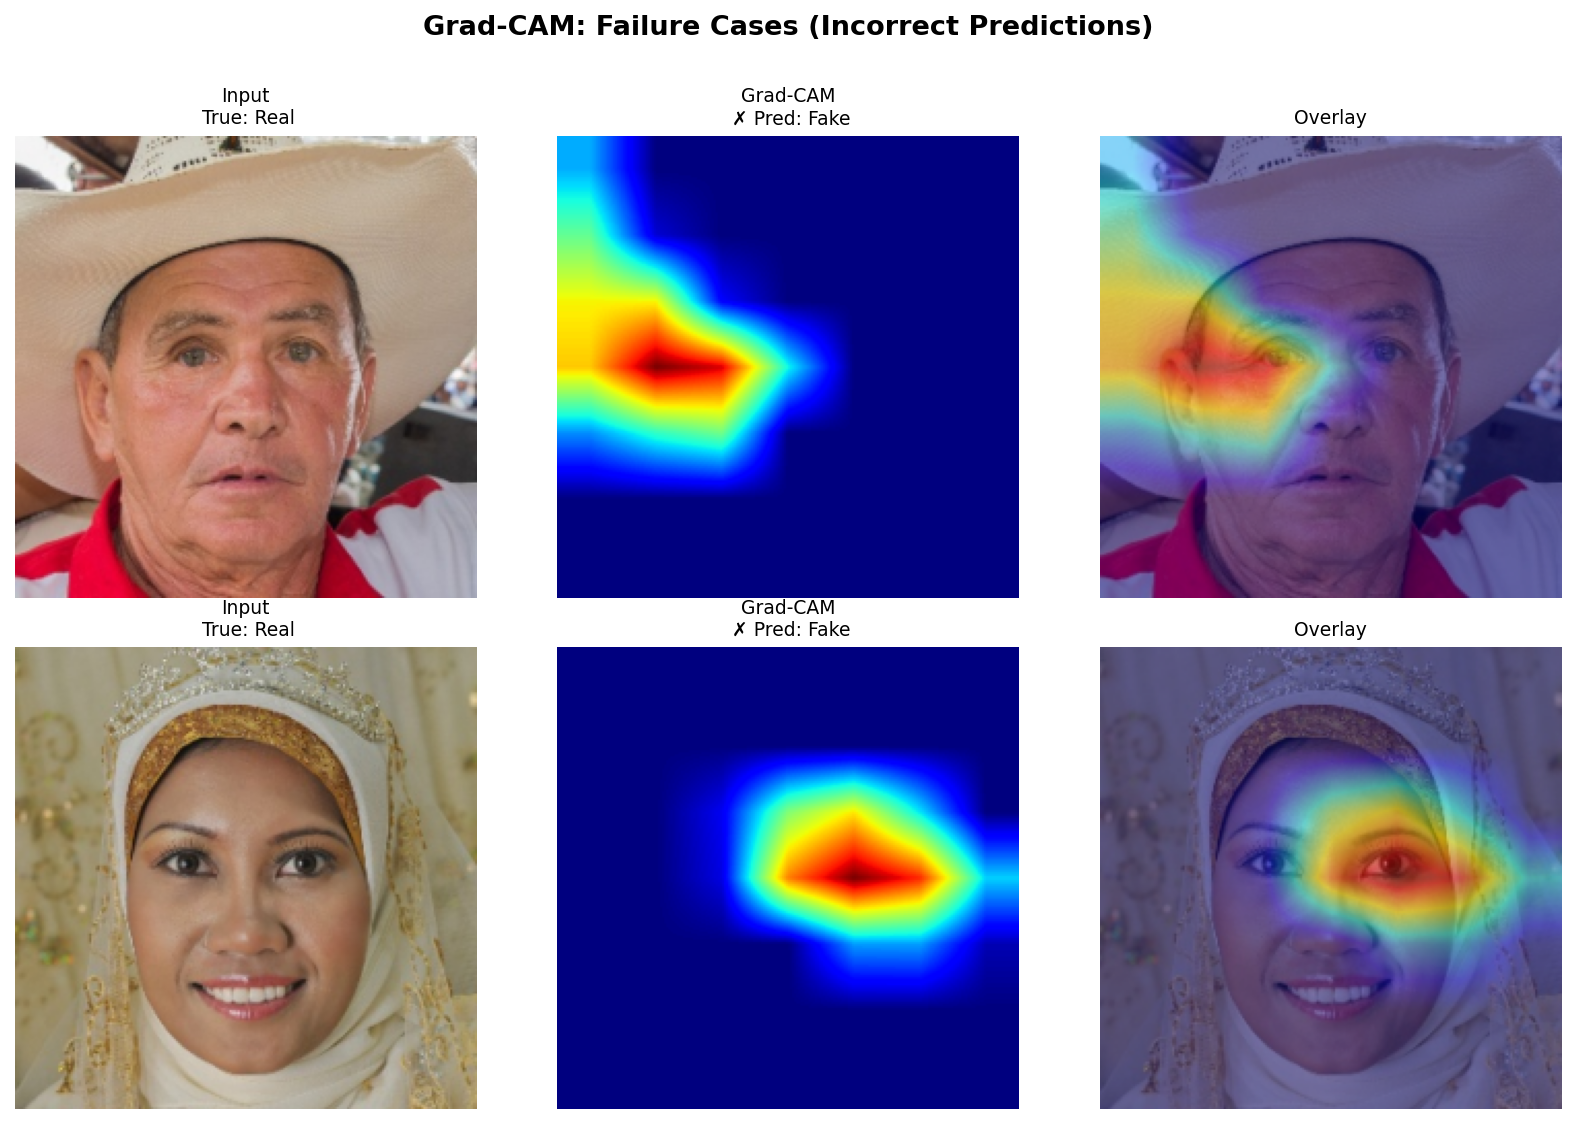
\includegraphics[width=\linewidth]{results/figures/gradcam_hybrid/gradcam_incorrect.png}
    \caption{Failure cases (real faces misclassified as fake).}
    \label{fig:gradcam_fail}
  \end{subfigure}
  \caption{%
    \textbf{Grad-CAM visualisations for the Hybrid model.}
    In every panel each row shows the input face (left), the Grad-CAM
    heatmap (middle), and the blended overlay (right).
    \textbf{(a)}~Correctly classified real faces — attention concentrates on
    central face-internal regions (eyes, nose, mouth).
    \textbf{(b)}~Misclassified real faces (predicted fake) — these cluster on
    images with unusual lighting, heavy cosmetics, or strong expression,
    surface patterns the model associates with GAN texture.
  }
  \label{fig:gradcam}
\end{figure*}

\section{Conclusion}
\label{sec:conclusion}

We designed and evaluated three CNN-based deepfake detectors on
StyleGAN2-generated face images.
Key findings:

\begin{enumerate}
  \item \textbf{FFT alone is insufficient.}  A ResNet18 on log-magnitude
    spectra achieves only 61\% accuracy (AUC\,=\,0.641) — barely above
    random — suggesting that StyleGAN2 spectral artefacts are not easily
    exploitable by a standard CNN at the scale studied.

  \item \textbf{RGB is a strong baseline.}  Fine-tuning a pretrained
    ResNet18 on raw face images yields 99\% accuracy (AUC\,=\,0.9975) with
    rapid convergence, confirming that ImageNet features transfer well to
    deepfake detection.

  \item \textbf{Hybrid outperforms both modalities.}  Late fusion achieves
    99.5\% accuracy, AUC\,=\,0.9998, and \emph{perfect recall} — the
    spectral branch resolves the residual ambiguous cases left by the
    spatial model.

  \item \textbf{Grad-CAM confirms interpretable attention.}  The RGB branch
    focuses on face-internal regions associated with GAN synthesis errors,
    providing evidence of genuine semantic learning.
\end{enumerate}

\paragraph{Limitations.}
The evaluation is limited to StyleGAN2 faces under clean conditions.
Frequency-based detectors are known to degrade under JPEG
compression~\cite{frank2020frequency}, and cross-generator
generalisation (to Stable Diffusion, FaceSwap, \etc) is untested.

\paragraph{Future work.}
Promising directions include: cross-generator robustness evaluation;
cross-attention fusion to replace naive concatenation; temporal consistency
modelling for video deepfake detection; and quantisation of the Hybrid model
for real-time deployment.

\paragraph{Acknowledgements.}
Dataset by Xhlulu~\cite{dataset140k} (Kaggle).
ImageNet weights via PyTorch \texttt{torchvision}.
Experiments run on a single NVIDIA GPU (CUDA 11.8 / 12.1).


% ── Bibliography ─────────────────────────────────────────────────────────────
{
    \small
    \bibliographystyle{ieeenat_fullname}
    \bibliography{main}
}

% Supplementary (not included in submission):
% \input{sec/X_suppl}

\end{document}
